%%%%%%%%%%%%%%%%%%%%%%%%%%
%%% author : Yamada. T %%%
%%% made for TH series %%%
%%%%%%%%%%%%%%%%%%%%%%%%%%

\documentclass[b5paper,10pt,fleqn] {ltjsarticle}

\usepackage[margin=10truemm]{geometry}

\usepackage{pict2e, graphicx}
\usepackage{tikz}
\usetikzlibrary{intersections,calc,arrows.meta}

\usepackage{amsmath, amssymb, amsthm}
\usepackage{ascmac}
\usepackage{comment}
\usepackage{empheq}
\usepackage[shortlabels,inline]{enumitem}
\usepackage{fancybox}
\usepackage{fancyhdr}
\usepackage{here}
\usepackage{lastpage}
\usepackage{listings, jvlisting}
\usepackage{fixdif}

\usepackage{stmaryrd}
\usepackage[listings]{tcolorbox}
%\usepackage{ascolorbox}
\usepackage{titlesec}
\usepackage{ulem}
\usepackage{url}
\usepackage{verbatim}
\usepackage{wrapfig}
\usepackage{xcolor}
\usepackage{luatexja-ruby}
\usepackage{varwidth}
\usepackage[version=3]{mhchem}
\usepackage{wrapfig}


\usepackage{physics2}
	\usephysicsmodule{ab}
	\usephysicsmodule{ab.braket}
	\usephysicsmodule{ab.legacy}
	%\usephysicsmodule{braket}
	\usephysicsmodule{diagmat}
	\usephysicsmodule{xmat}
	\usephysicsmodule{nabla.legacy}
	\usephysicsmodule{qtext.legacy}

\usepackage[ISO]{diffcoeff}
\difdef { f, s } { D }
{ op-symbol = \mathrm{D} }


\newcommand{\mctext}[1]{\mbox{\textcircled{\scriptsize{#1}}}}
\newcommand{\ctext}[1]{\textcircled{\scriptsize{#1}}}
\newcommand{\ds}{\displaystyle}
\newcommand{\comb}[2]{{}_{#1}\mathrm{C}_{#2}}
\newcommand{\hs}{\hspace}
\newcommand{\vs}{\vspace}
\newcommand{\emphvs}{\vspace{1em}\notag\\}
\newcommand{\ora}{\overrightarrow}
\newcommand{\ol}{\overline}
\newcommand{\oramr}[1]{\overrightarrow{\mathrm{#1}}}
\newcommand{\tri}{\triangle}
\newcommand{\mr}{\mathrm}
\newcommand{\mb}{\mathbb}
\newcommand{\mrvec}[1]{\overrightarrow{\mathrm{#1}}}
\newcommand{\itvec}{\overrightarrow}
\newcommand{\bs}{\boldsymbol}
\newcommand{\ra}{\rightarrow}
\newcommand{\Ra}{\Rightarrow}
\newcommand{\lra}{\longrightarrow}
\newcommand{\Lra}{\Longrightarrow}
\newcommand{\la}{\leftarrow}
\newcommand{\La}{\Leftarrow}
\newcommand{\lla}{\longleftarrow}
\newcommand{\Lla}{\Longleftarrow}
\newcommand{\lr}{\leftrightarrow}
\newcommand{\llr}{\longleftrightarrow}
\newcommand{\Llr}{\Longleftrightarrow}
\renewcommand{\deg}{{}^\circ}
\newcommand{\phbox}{\fbox{\phantom{1\hspace{2em}}}}
\newcommand{\boxnum}[1]{\fbox{\phantom{\hspace{1em}}({#1})\phantom{\hspace{1em}}}}
\newcommand{\boxkana}[1]{\fbox{\phantom{\hspace{1em}}{#1}\phantom{\hspace{1em}}}}
\newcommand{\boxkm}[2]{\fbox{\, {#1}\phantom{\hspace{0.2em}} \,  {#2}}}
\newcommand{\hzw}{\hspace{1\zw}}

\renewcommand{\baselinestretch}{1.25}
\parindent=1\zw

\begin{document}
\noindent\fbox{NewTH1-4} [名古屋大]

図1のように,ばねによって発射される小物体の運動を考える.
小物体の質量は$m$であり,大きさが無視できる.
ばねは,一端が固定されて,他端に板が取り付けられている.
ばねはフックの法則に従い,ばね定数を$k$とする.
空気抵抗,ばねおよび板の質量は無視できるのものとする.
重力は鉛直下向きにはたらき,重力加速度の大きさを$g$とする.
すべての運動は,図1に示す鉛直平面内で起こるものとする.以下の設問に答えよ.
計算欄には,答に至るまでの過程の\textbf{要点}(法則,関係式,論理,計算など)を書け.


\begin{figure}[H]
  \centering
  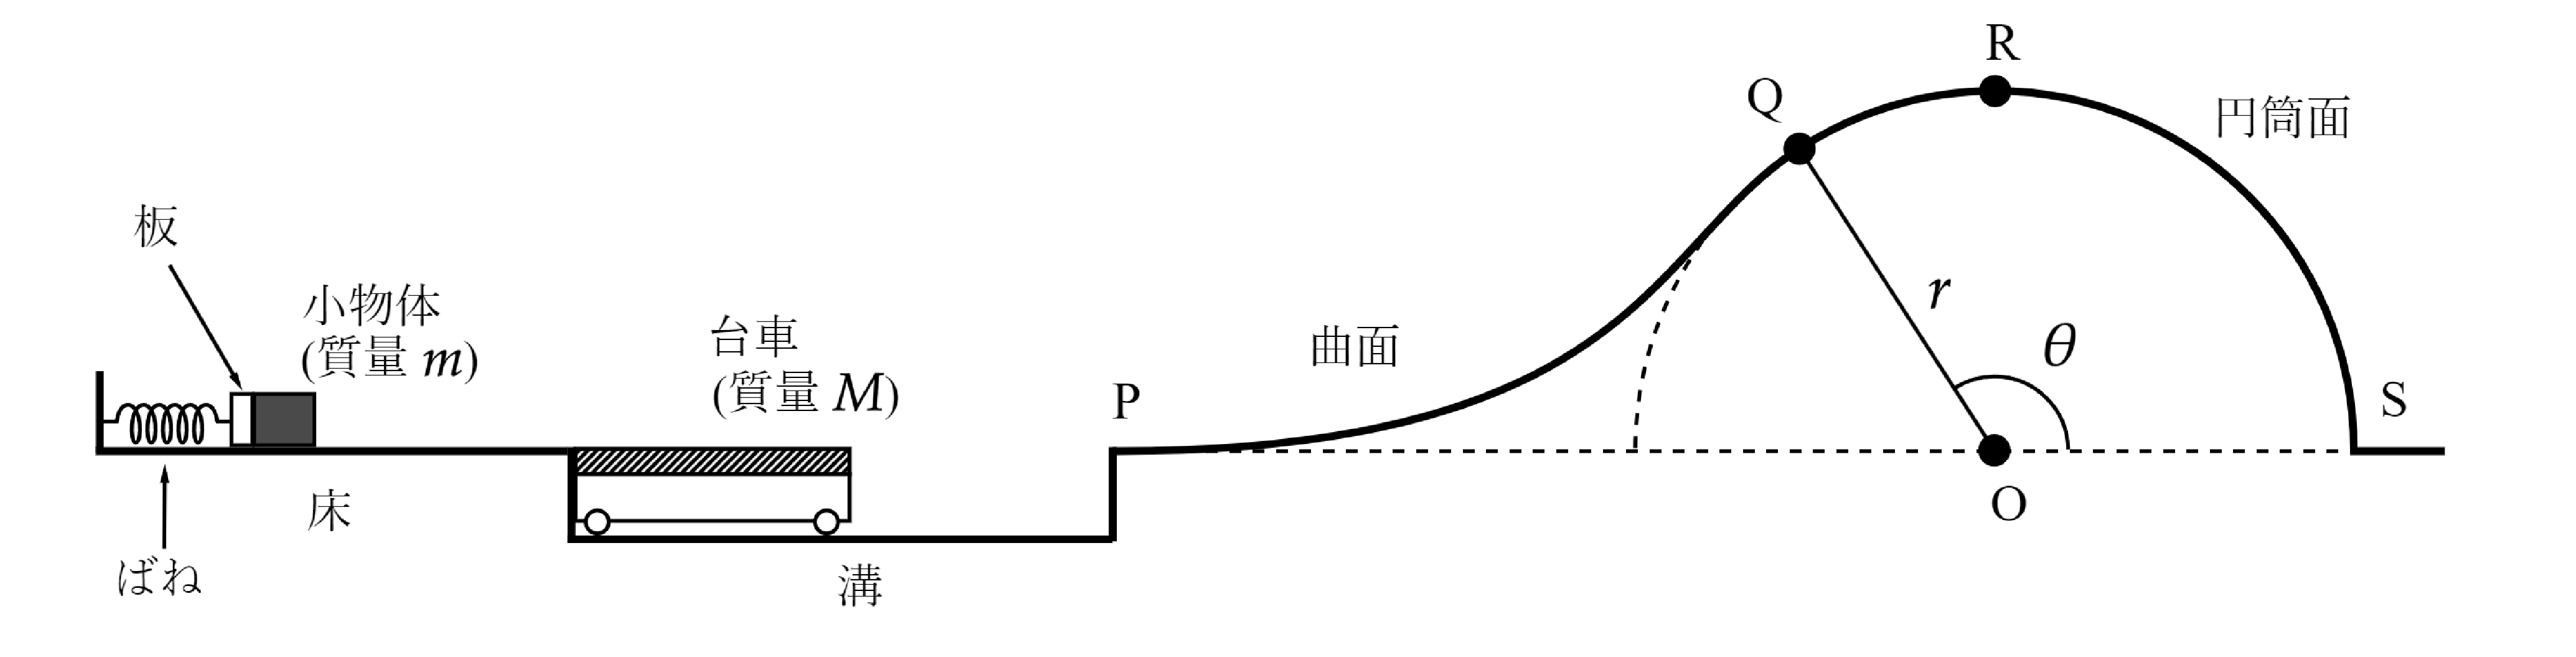
\includegraphics[width=12cm]{fig/fig_1_4.pdf}
\end{figure}

ばねが自然長から$d$だけ縮むように小物体を押し,静かに放した.
小物体は,板から離れて,水平な床を右向きに速さ$v_0$で運動した.
床と小物体との間の摩擦は無視できるものとする.

\begin{enumerate}[label={\textbf{問\arabic*}}]
  \item \hzw 速さ$v_0$を,$m$,$d$,$g$,$k$の中から適切なものを用いて表せ.
\end{enumerate}
床の右側には水平な溝が掘ってある.
この溝の左端に,質量$M$の台車が静止している.
台車の上面は水平であり.床と同じ高さにある.

小物体が床から台車に乗り移った後,小物体と台車はいずれも右向きに運動した.
台車に乗り移った直後の小物体の速さは$v_0$であった.
台車の上面と小物体との間には,摩擦があり,その動摩擦係数を$\mu'$とする.
台車の右端と小物体は,同時に同じ速さ$v_1$で溝の右端に到達した.
台車と溝との間の摩擦は無視できるものとする.
\begin{enumerate}[resume, label={\textbf{問\arabic*}}]
  \item {\hzw}小物体が台車上を運動しているとき,小物体と台車の加速度(右方向を正)を,それぞれ$a$,$A$とする.
  
  {\hzw}小物体と台車の水平方向の運動方程式を,それぞれ
  $m$,$M$,$v_0$,$a$,$A$,$g$,$\mu'$の中から適切なものを用いて記せ.

  \item {\hzw}速さ$v_1$を,$m$,$M$,$v_0$,$g$,$\mu'$の中から適切なものを用いて表せ.
\end{enumerate}
曲面PQがなめらかに円筒面QSにつながっている.円筒面QSの中心はO,その半径は$r$である.円筒の軸は,小物体が運動する鉛直平面に垂直である.P,O,Sの各点は,床と同じ高さにある.円筒面QSの最高点をRとする.$\angle \mr{QOS} = \theta \ (\theta > 90\deg)$とする.

小物体は,台車から曲面に乗り移り,曲面および円筒面から離れずにRに到達した.Qを通過した直後の円筒面上での小物体の速さを$v_2$とし,このときの円筒面からの垂直抗力の大きさを$N$とする.Rでの小物体の速さを$v_2$とする.曲面および円筒面と小物体の間の摩擦は無視できるものとする.
\begin{enumerate}[resume, label={\textbf{問\arabic*}}]
  \item {\hzw}速さ$v_2$を,$m$,$M$,$r$,$\theta$,$v_2$,$g$の中から適切なものを用いて表せ.
  \item {\hzw}垂直抗力の大きさ$N$を,$m$,$M$,$r$,$\theta$,$v_2$,$g$の中から適切なものを用いて表せ.
  \item {\hzw}小物体が,円筒面から離れずに,最高点Rに到達するための速さ$v_2$の条件を$m$,$M$,$r$,$\theta$,$g$の中から適切なものを用いて表せ.
\end{enumerate}
\end{document}